\documentclass[14pt, letterpaper, oneside]{extarticle}
\usepackage{graphicx}
\usepackage{float}
\usepackage[margin=1in]{geometry}
\usepackage{parskip}
\usepackage{listings}
\usepackage{hyperref} 
\usepackage{array}
\usepackage{tabularx}
\newcolumntype{Y}{>{\centering\arraybackslash}X}

\begin{document}
% chktex-file 44

\begin{titlepage}
    \vspace*{\fill} %
    \centering
    {\Huge \textbf{CS 2850} \par}
    {\vspace{2cm}}
    {\LARGE By Tony Song \par}
    {\vspace{2cm}}
    {\LARGE August 2025 \par}
    \vspace*{\fill}
\end{titlepage}

\newpage
\tableofcontents

\newpage
\section{Mon 8/25}
\subsection{Course info}

One review class before before each prelim. One review class before final.

Suggest going to at least one TA sessions

Not punished for using AI, but def won't help learn

Exams are completely closed book

Usually, homeworks are out on Monday. Need to submit homework by \textbf{11:59 PM on Sundays}.
HW is still taken 24 hours after but with 10\% off. HW is rejected after 24 hours 

\subsection{Networks}
Network:

\textbf{Nodes} (representing a person)

\textbf{Link} (representing connections between two people)

Inferences based on network info:
\begin{enumerate}
    \item Who is the leader (people with the most connections)
    \item Which one of the two parties an individual is more likely to side with
\end{enumerate}

Networks can model the progression of (the spread of) a flu contagion

The shortest route is technically a straight line. GMaps gives the user a detour, however.

But the user has to travel on the network, a composition of a roads and paths.

Every intersection is a \textbf{node}. Every main road is one type of \textbf{link}. Every \textit{other} road is another type of \textbf{link}

Systemic risk:
If a node (A) is a large net seller, and (A) goes bankrupt, then every node in the network (even linked indirectly) can go bust.

Don't have to be a large node yourself. You are also systemic if you are linked with the big nodes.

If a node is dominant in connections, then they are \textbf{central}. There is some sort of \textbf{centrality} to it.

Besides finance, networks are also very relevant in politics.

Each node is a blog. Each link indicates a reference to a connected blog.

\section{Wed 8/27}
\subsection{Graph Theory}
Graph: a way of specifying relationships among a collection of items
Collection of items: nodes
Relationships: edges/links

\begin{tabularx}{\textwidth}{Y|Y}
    Collection of items & relationship \\
    \hline
    People & friendship \\
    Institutions & borrow-lender \\
    Products & proximity \\
    Organism & predator-prey
\end{tabularx}

Symmetric relationship:
A is B's friend = B is A's friend

A graph that has \textbf{symmetric} relationship is an \textbf{undirected} network

Assymetric relationship: A follows B $\neq$ B follow A

A graph that has \textbf{assymmetric} relationship is an \textbf{undirected} network

\subsubsection{Degree}
Degree: the number of connections (edges) a node has to other nodes

In a network of n nodes and m edges, $0 \leq$ Degree $\leq n - 1$

Sum of degrees $= 2m$

Think about handshakes. 

Imagine a classroom of 10 people. Each person shakes hands with exactly 3 others:

So $10 \times 3 = 30$ total degrees = $30 \div 2 = 15$ edges / handshakes

Could a graph exist where every node has degree 3, but the total number of nodes is 5?
No. Total degrees $= 3 \times 5 = 15$. Links = $15 / 2 = 7.5$ edges. Have to be integer.

\subsubsection{Path}
Path: a sequence of nodes, where each conseuctive pair of nodes is connected by an edge

You are techniicaly allowed to go back and forth between two nodes.

Length of a path: number of steps it contains from beginning to end.

We are interested in the shortest path between two nodes

\section{Fri 8/29}
\subsection{Strong and Weak Ties}
A graph is \textbf{``connected''} if \textit{each pair} of nodes can be connected through a path

It can still be decomposed into \textbf{connected components}.

Two nodes are connected through a path \textbf{if and only} if they are in the same connected component.

If two nodes are in the same connected component, there is always a path connecting the two

If two nodes are in different connected components, there is never a path connecting the two

\begin{figure}[H]
    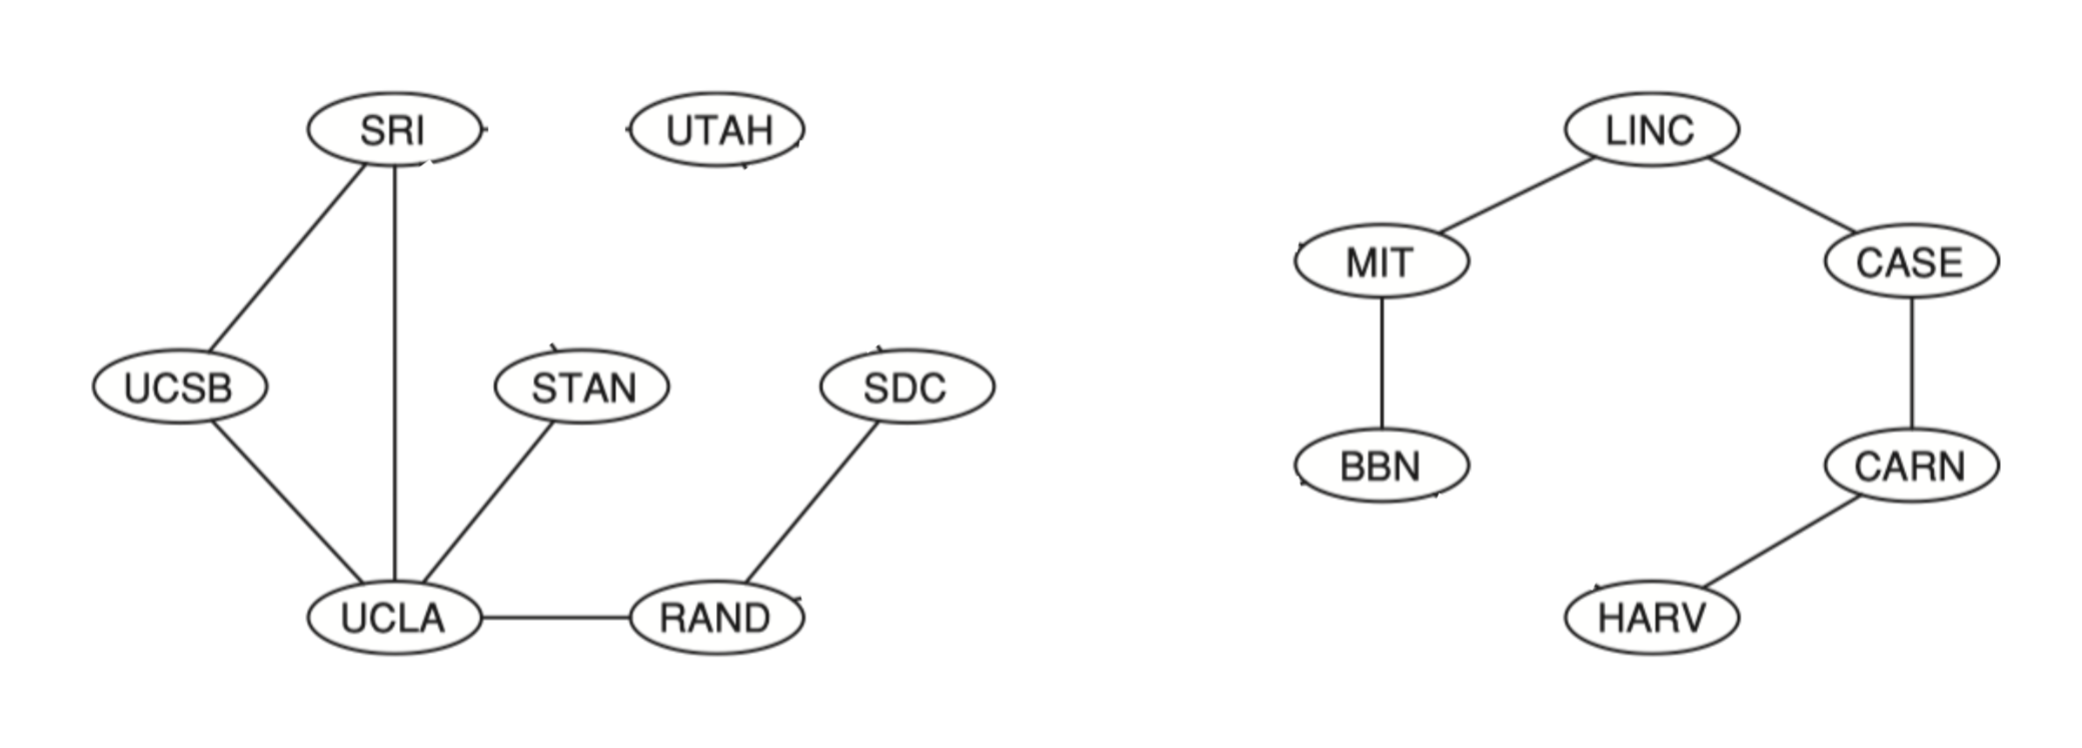
\includegraphics[width=0.8\textwidth]{images/1}
    \caption{An isolated node is also a connected component}
\end{figure}

\textbf{Bridge}: An edge connecting x and y is called a bridge if deleting it would cause x and y to lie in two
different components — the only path between x and y.

\textbf{Local bridge}: An edge connecting x and y is called a local bridge if deleting it would cause x and y to have a
distance > 2 — no common friends between x and y.

\textbf{Bridges are always local bridges}
 

\section{Wed 9/3}
\subsection{Strong and Weak Ties}

Strong Tradic closure (STC): If node a has strong ties to nodes B and C, then the B-C edge if \textit{very} likely to form

A node \textbf{satisfies} STC property if every two of its strong tie friends are also friends (all of strong-tie friends must know each other), OR if it has less than two strong tie friends.

Otherwise it \textbf{violates} STC property

\begin{figure}[H]
    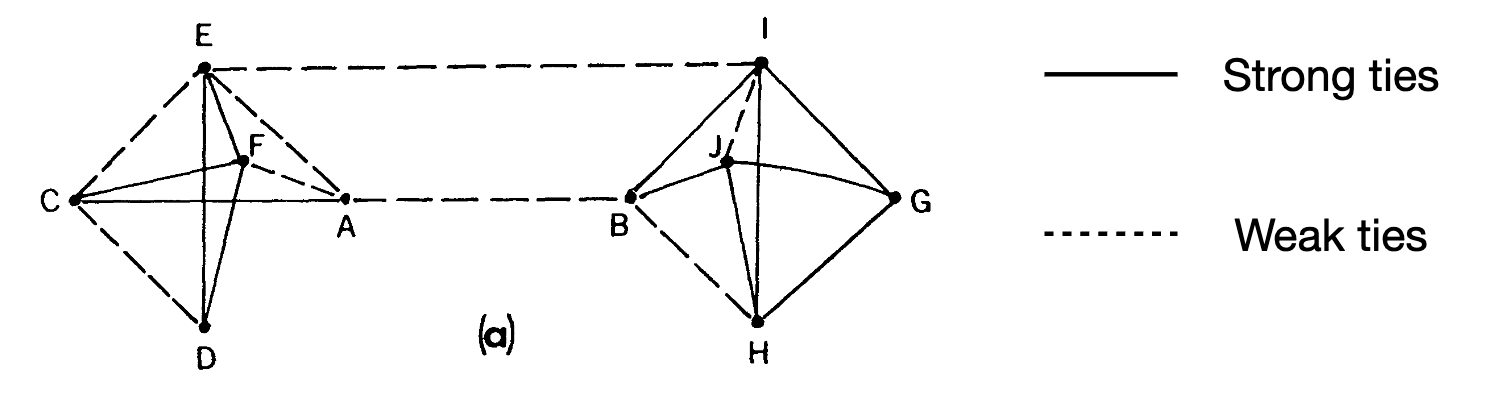
\includegraphics[width=0.8\textwidth]{images/2}
    \caption{A and D satify the STC property, while J does not}
\end{figure}

Any local bridge must be a weak tie.

Weak ties are not neccessarily worse than strong tie. Strong ties likely result in receiving the same information.

When trying to find a job, weak ties might would be more helpful. What is important is a diverse collection of strong and weak ties.

\subsection{Labeled Networks}
Does not make sense to label enemies with the same edge as friends

\begin{figure}[H]
    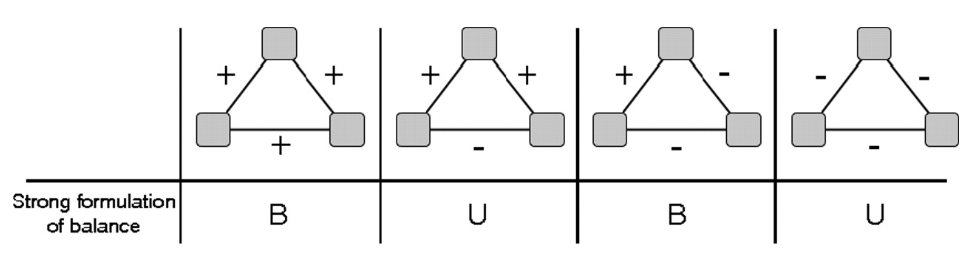
\includegraphics[width=0.8\textwidth]{images/3}
    \caption{Second and fourth triangles are unbalanced (uncommon in society). In triangle 2, the common friend would likely have to take a side,
    resulting in triangle 3. In triangle 4, having common enemies can result in a mutual friend, as in triangle 3}.
\end{figure}

\section{Fri 9/5}

\end{document}
